%%=============================================================================
%% Methodologie
%%=============================================================================

\chapter{\IfLanguageName{dutch}{Methodologie}{Methodology}}%
\label{ch:methodologie}

Deze bachelorproef zal bestaan uit 4 grote fasen: het uitvoeren van een literatuurstudie, een toelichting van de gebruikte technologieën en tools, het opzetten van een proof-of-concept (PoC) en tot slot het uitvoeren van de testen en het evalueren van de resultaten. Hieronder zal elke fase in detail besproken worden alsook het doel van de fase samen met de uitwerking ervan.

\section{Literatuurstudie uitvoeren}

De eerste fase van deze bachelorproef bestaat uit een literatuurstudie. Hierin zal aan de hand van diverse bronnen een beeld gegeven worden over de huidige stand van zaken omtrent het onderwerp van deze bachelorproef.\newline 

In het eerste hoofdstuk van deze studie wordt de monolithische architectuur besproken. Dit hoofdstuk definieert wat een monolithische applicatie is, wat de opbouw ervan is en welke voor- en nadelen deze architectuur met zich meebrengt. Hierbij zal er gekeken worden naar de typische gelaagde structuur (presentatielaag, businesslaag en datalaag). Vervolgens wordt de aandacht gegeven aan de microservices-architectuur. Dit hoofdstuk geeft een definitie en kenmerken van microservices, waarbij er voornamelijk zal gefocust worden op de onafhankelijkheid van services, de manier van communicatie en de impact op schaalbaarheid en onderhoud. Daarnaast worden enkele belangrijke principes van microservices aangehaald. Door deze architectuur te vergelijken met monolithische applicaties, wordt duidelijk beeld gegeven van de voordelen en uitdagingen van een microservices-architectuur.\newline

Naast de bespreking van monolithische en microservices-architecturen worden in de literatuurstudie ook enkele relevante termen onder de loep genomen. Allereerst wordt er gekeken naar gedistribueerde systemen die basis vormen voor moderne softwarearchitecturen, zoals de microservices en Service-Oriented Architecture (SOA). Daarnaast wordt dieper ingegaan op het concept van een Enterprise Service Bus (ESB) als communicatiemechanisme binnen SOA. Gevolgd door de verschillen tussen SOA en microservices. Polyglot persistence wordt besproken als een strategie om verschillende databases te combineren op basis van specifieke behoeften. Tot slot wordt er nog gekeken naar Docker en Kubernetes als tools voor containerisatie bij het uitwerken van de microservices.

\section{Tools en technologieën}
\label{tools_en_technologieën}

Voor de proof-of-concept (PoC) wordt er zowel een monolithische als een microservices-applicatie ontwikkeld. In de literatuurstudie werd vastgesteld dat er een vrijheid is in de keuze van technologieën bij het ontwikkelen van microservices. Dit hoofdstuk bespreekt de gekozen tools en technologieën die gebruikt zullen worden voor de implementatie van beide applicaties.

\subsection{Programmeertaal en framework}

Voor het ontwikkelen van de applicaties wordt C\# samen met .NET 8 gebruikt. .NET 8 biedt integratiemogelijkheden met containertechnologieën zoals Docker en Kubernetes, maar ook ondersteuning voor moderne communicatiemechanismen zoals RabbitMQ.

\subsection{Containerisatie en orkestratie}

Docker zal gebruikt worden om de applicaties, samen met z'n dependencies, te verpakken als containers. Hierdoor kunnen de applicaties makkelijk op diverse systemen gebruikt worden. Voor het beheren van de microservices wordt Kubernetes gebruikt. Kubernetes biedt uitgebreide mogelijkheden voor het automatisch schalen, distribueren en herstellen van containers, wat zorgt voor een robuuste en flexibele microservices-architectuur.

\subsection{Communicatie}

Voor de communicatie tussen de diverse services van de microservices-applicatie zal volgend communicatiemechanisme gebruikt worden:

\begin{itemize}
	\item \textbf{RabbitMQ} - RabbitMQ maakt het mogelijk om berichten asynchroon uit te wisselen tussen verschillende services. Dit zorgt voor een losse koppeling tussen services, waardoor ze onafhankelijk van elkaar kunnen functioneren en schalen. RabbitMQ ondersteunt betrouwbare berichtafhandeling, berichtvolgorde en verschillende berichtpatronen zoals publish/subscribe, wat het bijzonder geschikt maakt voor microservices-architecturen waarin flexibiliteit en schaalbaarheid cruciaal zijn.
\end{itemize}

\subsection{Database}

Tot slot voor de database is er ook volgens het polyglot persistence principe een vrijheid in welke type database er gekozen wordt. Voor de eenvoud van deze PoC zal er gekozen worden voor SQL Server. Zowel de monolithische als de microservices-applicatie zullen dezelfde database-engine gebruiken. Bij de microservices krijgt elke service een eigen, aparte database.

\section{Opzetten van PoC}
\label{opzetten_poc}

In de derde fase van deze bachelorproef zal een proof-of-concept (PoC) uitgewerkt worden om de theorie en inzichten uit de literatuurstudie om te zetten in een uitwerkt voorbeeld. Het doel van deze PoC is om de verschillen tussen een monolithische architectuur en een microservices-architectuur op vlak van schaalbaarheid en complexiteit te analyseren.

Hiervoor zullen twee versies van een e-commerce applicatie ontwikkeld worden. De eerste zal een monolithische architectuur hebben met alle functionaliteiten in één codebase. De tweede zal de microservices-architectuur implementeren waarbij de functionaliteiten zullen opgesplitst worden in services die apart draaien in kubernetes. De \hyperref[tools_en_technologieën]{tools en technologieën} die gebruikt zullen worden zijn hierboven aangekaart.

\section{Testen en resultaten}

Vervolgens zullen er testen worden uitgevoerd op de twee applicaties. Allereerst wordt de schaalbaarheid van beide applicaties getest met behulp van Apache JMeter. Deze gratis open-source software maakt het mogelijk om simulaties van hoge belasting uit te voeren, zodat de prestaties onder intensief gebruik van beide applicaties kunnen vergeleken worden. Daarnaast wordt de complexiteit beoordeeld door het meten van de cyclomatische complexiteit. Hiervoor zal er gebruik gemaakt worden van de gratis versie van SonarQube. Met behulp van deze tool wordt een grondige code analyse uitgevoerd om een beeld te krijgen van de complexiteit van de applicaties.

Tot slot zullen de resultaten van de Apache JMeter testen en de SonarQube analyse worden gebruikt om een conclusie te trekken over de schaalbaarheid en complexiteit van de microservices-architectuur ten opzichte van de monolithische aanpak om aan te tonen of er weldegelijk een optimalisatie is.




\chapter{\IfLanguageName{dutch}{Uitwerking}{Elaboration}}%
\label{ch:uitwerking}

In dit hoofdstuk wordt de technische uitwerking van de proof-of-concept (PoC) besproken. Zoals eerder aangehaald, bestaat deze PoC uit twee versies van een simpele e-commerce applicatie: één met een monolithische architectuur en één met een microservices-architectuur. Het doel van dit hoofdstuk is om stap voor stap de implementatie van beide applicaties te bespreken. Hierbij zal gekeken worden naar de architecturale keuzes, de gebruikte tools en technologieën, en de manier waarop de verschillende services van het systeem met elkaar interageren.

\section{Overzicht van de functionaliteiten}

Voor de uitwerking van de proof-of-concept werd gekozen om een vereenvoudigde e-commerce applicatie te ontwikkelen. Dit type applicatie omvat diverse bedrijfsprocessen. Zowel de monolithische als de microservices-applicatie zullen dezelfde functionaliteiten implementeren, zodat in een later stadium de applicatie eerlijk vergeleken kunnen worden op vlak van schaalbaareid.

\subsection{Gekozen functionaliteiten}

Hieronder volgt een overzicht van de kernfunctionaliteiten voor beide applicaties:

\begin{itemize}
	\item \textbf{Gebruikersbeheer}
	\begin{itemize}
		\item Registreren van nieuwe gebruikers
		\item Inloggen en authenticatie
	\end{itemize}
	\item \textbf{Productbeheer}
	\begin{itemize}
		\item Lijst van beschikbare producten raadplegen
		\item CRUD-operaties op producten
	\end{itemize}
	\item \textbf{Winkelwagen en bestelling}
	\begin{itemize}
		\item Producten toevoegen aan winkelwagen
		\item Bezichtigen van winkelwagen
		\item Plaatsen van een bestelling (winkelwagen legen)
		\item Raadplegen van geplaatste bestellingen per gebruiker
	\end{itemize}
\end{itemize}

Deze functionaliteiten zorgen ervoor dat bij een microservices-applicatie nagedacht moet worden over een logische opdeling in afzonderlijke services. Zo kunnen bijvoorbeeld een User Service, Product Service, ShoppingCart Service en Order Service geïmplementeerd worden. Dit resulteert in een omgeving waarin een zekere mate van samenwerking tussen services nodig is. Hierdoor kunnen verschillende communicatiepatronen worden toegepast, zoals synchrone en asynchrone communicatie (bijv. via RabbitMQ).

\section{Implementatie van de monolithische applicatie}

In dit onderdeel van hoofdstuk 4 wordt de implementatie van de monolithische versie van de e-commerce applicatie besproken. Zoals beschreven in het \hyperref[opzetten_poc]{opzetten van de PoC} wordt deze versie volledig uitgewerkt binnen één codebase, waarbij alle functionaliteiten centraal beheerd worden. De applicatie werd ontworpen met C\# in combinatie met het .NET 8 framework.

\subsection{Architectuur en projectstructuur}

De monolithische applicatie werd opgebouwd als een ASP.NET Core Web API. Alle functionaliteiten zijn aanwezig binnen één projectstructuur en communiceren rechtstreeks met dezelfde database. Figuur \ref{fig:Docker vs VM} illustreert de architectuur van de eerste applicatie.

\begin{figure}[H]
	\centering
	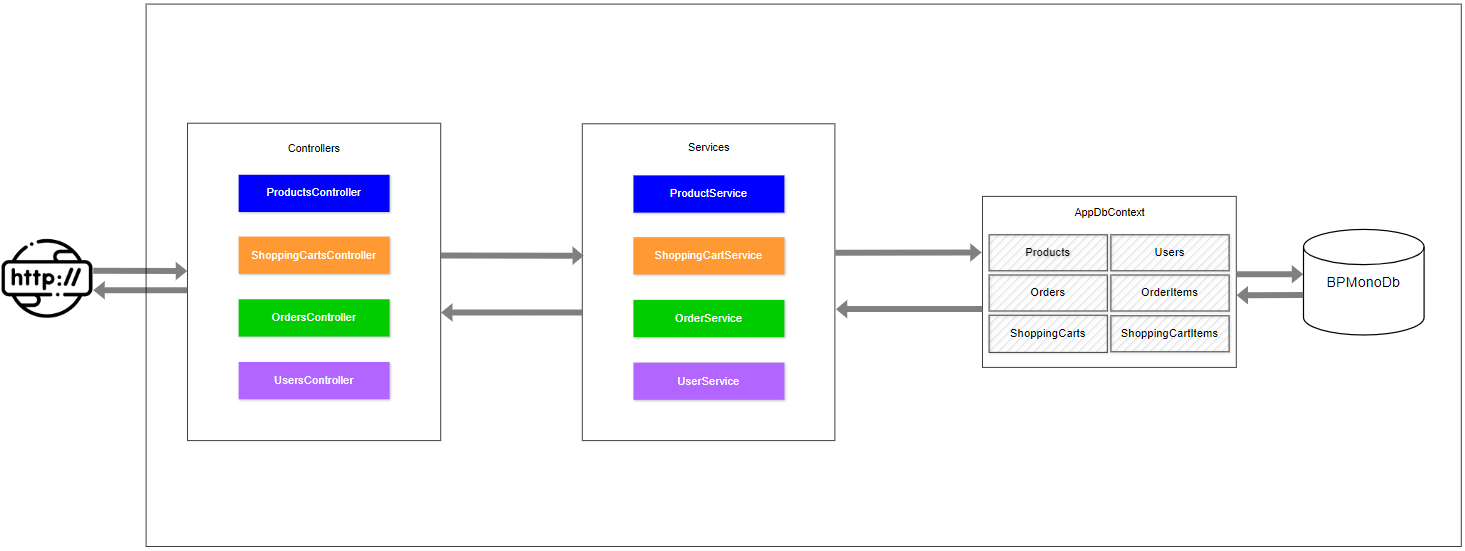
\includegraphics[width=1\textwidth]{BPMono.png}
	\caption[Voorstelling van de monolithische architectuur voor de PoC.]{\label{fig:BPMono}Voorstelling van de monolithische architectuur voor de PoC.\linebreak}
\end{figure}

De projectstructuur bevat verschillende mappen die de lagen logisch scheiden:

\begin{itemize}
	\item \textbf{Auth} - Bevat de logica voor authenticatie, waaronder een JWT-token provider voor het genereren van tokens en een wachtwoord-hasher om wachtwoorden veilig op te slaan.
	\item \textbf{Controllers} – Definiëren API-endpoints die inkomende HTTP-verzoeken van de client afhandelen en doorsturen naar de correcte services.
	\item \textbf{Data} - Omvat de AppDbContext klasse voor de database via Entity Framework Core en methodes voor het seeden van data.
	\item \textbf{Models} – Bevat domeinmodellen die de database-entiteiten representeren.
	\item \textbf{DTOs} – Data Transfer Objects die worden gebruikt om data uit te wisselen tussen de client en de server. 
	\item \textbf{Profiles} - Bevat AutoMapper-profielen die verantwoordelijk zijn voor het automatisch mappen van domeinmodellen naar DTO's en omgekeerd.
	\item \textbf{Services} – Implementeren van businesslogica en interacties met de database.
\end{itemize}

\subsection{Productbeheer}

Het productbeheer is een belangrijk onderdeel van de applicatie. Zonder producten kan de winkelwagen niets bevatten en kan er geen bestelling worden geplaatst. Hieronder volgt een voorbeeld van hoe producten beheerd worden binnen de monolithische architectuur. De \texttt{ProductsController} bevat endpoints voor CRUD-operaties, die dan gebruikmaken van de \texttt{ProductService}.

\medskip
Het eerste fragment toont het \texttt{Product}-model. Dit model representeert de structuur van een product zoals die in de database wordt opgeslagen. Elk product heeft een unieke ID, een naam en een prijs. De attributen zijn geannoteerd met data-anotaties voor validatie en database-constraints.
\medskip

\begin{lstlisting}[style=mystyleA, caption=Product.cs, label=lst:MonoProductModel]
public class Product
{
	[Key]
	[Required]
	public int Id { get; set; }
	
	[Required]
	public string Name { get; set; }
	
	[Required]
	public double Price { get; set; }
}
\end{lstlisting}

\medskip
De \texttt{ProductsController} bevat de API-endpoints waarmee de client producten kan opvragen. In het onderstaande fragment is het GET-endpoint weergegeven dat alle producten ophaalt. Dependency injection wordt gebruikt om de service en mapper te injecteren. De producten worden via de service opgehaald uit de database, en vervolgens gemapt naar \texttt{ProductReadDto}-objecten met AutoMapper.
\medskip

\begin{lstlisting}[style=mystyleA, caption=ProductsController.cs (fragment), label=lst:MonoProductsController]
[Route("api/[controller]")]
[ApiController]
[Authorize]
public class ProductsController : ControllerBase
{
	private readonly IProductService _service;
	private readonly IMapper _mapper;
	
	public ProductsController(IProductService service, IMapper mapper)
	{
		_service = service;
		_mapper = mapper;
	}
	
	[HttpGet]
	public async Task<ActionResult<List<ProductReadDto>>> GetProducts()
	{
		Console.WriteLine("--> Getting all products...");
		var products = await _service.GetAllProducts();
		if (products == null)
			return NotFound("No products found");
		return Ok(_mapper.Map<List<ProductReadDto>>(products));
	}
}
\end{lstlisting}

\medskip
Tot slot wordt hieronder de implementatie van de \texttt{ProductService} weergegeven. Deze service maakt gebruik van Entity Framework Core om via de \texttt{AppDbContext} alle producten op te halen uit de database.
\medskip

\begin{lstlisting}[style=mystyleA, caption=ProductService.cs (fragment), label=lst:MonoProductService]
public class ProductService(AppDbContext context) : IProductService
{
	private readonly AppDbContext _context = context;
	
	public async Task<List<Product>> GetAllProducts()
	{
		return await _context.Products.ToListAsync();
	}
}
\end{lstlisting}

\subsection{Winkelwagen}

Gebruikers kunnen met de winkelwagen producten bijhouden voordat deze in een bestelling worden omgezet.

\medskip
Het \texttt{ShoppingCart}-model stelt een winkelwagen voor die gekoppeld is aan een gebruiker via een \texttt{UserId}. Elke winkelwagen bevat een verzameling \texttt{ShoppingCartItem}-objecten, die de producten in de winkelwagen voorstellen.
\medskip

\begin{lstlisting}[style=mystyleA, caption=ShoppingCart.cs, label=lst:MonoShoppingCartModel]
public class ShoppingCart
{
	[Key]
	[Required]
	public int Id { get; set; }
	
	[Required]
	public int UserId { get; set; }
	
	public IEnumerable<ShoppingCartItem> Items { get; set; }
}
\end{lstlisting}

\medskip
Het \texttt{ShoppingCartItem}-model vormt de link tussen de producten en een gebruikers winkelwagen. Elk item verwijst naar zowel een \texttt{ShoppingCart} als een \texttt{Product}. Dit model maakt het mogelijk om meerdere producten aan één winkelwagen toe te voegen.
\medskip

\begin{lstlisting}[style=mystyleA, caption=ShoppingCartItem.cs, label=lst:MonoShoppingCartItemModel]
public class ShoppingCartItem
{
	[Key]
	[Required]
	public int Id { get; set; }
	
	[Required]
	public int ShoppingCartId { get; set; }
	
	[Required]
	public int ProductId { get; set; }
	
	[ForeignKey("ShoppingCartId")]
	public ShoppingCart ShoppingCart { get; set; }
	
	[ForeignKey("ProductId")]
	public Product Product { get; set; }
}
\end{lstlisting}

\medskip
De \texttt{ShoppingCartsController} bevat naast een GET-endpoint ook een PUT-endpoint om een product toe te voegen aan de winkelwagen van de ingelogde gebruiker. De \texttt{UserId} wordt uit de JWT-token van de gebruiker gehaald.
\medskip

\begin{lstlisting}[style=mystyleA, caption=ShoppingCartsController.cs (fragment), label=lst:MonoShoppingCartController]
[Route("api/[controller]")]
[ApiController]
[Authorize]
public class ShoppingCartsController : ControllerBase
{
	private readonly IShoppingCartService _shoppingCartService;
	private readonly IProductService _productService;
	private readonly IMapper _mapper;
	
	public ShoppingCartsController(IShoppingCartService shoppingCartService, IProductService productService, IMapper mapper)
	{
		_shoppingCartService = shoppingCartService;
		_productService = productService;
		_mapper = mapper;
	}
	
	[HttpPut("{productId}")]
	public async Task<ActionResult> AddProductToCart(int productId)
	{
		Console.WriteLine("--> Adding a product...");
		var userIdClaim = User.FindFirst(ClaimTypes.NameIdentifier)?.Value;
		if (string.IsNullOrEmpty(userIdClaim) || !int.TryParse(userIdClaim, out int userId))
			return Unauthorized("UserId kon niet worden bepaald uit JWT token");
		
		try
		{
			await _shoppingCartService.AddProductToCart(userId, productId);
			return Ok($"Product {productId} added to cart for user {userId}");
		}
		catch (Exception ex)
		{
			return BadRequest($"Failed to add product {productId} to cart of user {userId}: {ex.Message}");
		}
	}
}
\end{lstlisting}

\medskip
De methode uit de \texttt{ShoppingCartService} bevat de logica om een product toe te voegen aan de winkelwagen van een specifieke gebruiker. Indien de winkelwagen nog niet bestaat voor de gebruiker, wordt er een nieuwe aangemaakt. Vervolgens wordt er een \texttt{ShoppingCartItem} toegevoegd met een verwijzing naar het product.
\medskip

\begin{lstlisting}[style=mystyleA, caption=ShoppingCartService.cs (fragment), label=lst:MonoShoppingCartService]
public class ShoppingCartService(AppDbContext context, IProductService productService) : IShoppingCartService
{
	private readonly AppDbContext _context = context;
	public readonly IProductService _productService = productService;
	
	public async Task AddProductToCart(int userId, int productId)
	{
		if (!await _context.Products.AnyAsync(p => p.Id == productId))
		throw new Exception($"No product found with id {productId}");
		
		var cart = await GetCart(userId);
		if (cart == null)
		{
			cart = new ShoppingCart { UserId = userId };
			_context.ShoppingCarts.Add(cart);
			await _context.SaveChangesAsync();
		}
		
		var cartItem = new ShoppingCartItem
		{
			ShoppingCartId = cart.Id,
			ProductId = productId
		};
		_context.ShoppingCartItems.Add(cartItem);
		await _context.SaveChangesAsync();
	}
}
\end{lstlisting}

\subsection{Bestellingen}

Wanneer een gebruiker beslist om de producten in de winkelwagen te bestellen, wordt er een bestelling aangemaakt. Deze bestelling bevat de producten uit de winkelwagen, berekent het totaalbedrag en slaat de bestelling op in de database.

\medskip
Het \texttt{Order}-model stelt een bestelling voor die gekoppeld is aan een gebruiker via een \texttt{UserId}. Elke bestelling bevat een lijst van \texttt{OrderItem}-objecten, samen met de totale prijs en een status dat de progressie van de bestelling bijhoudt.
\medskip

\begin{lstlisting}[style=mystyleA, caption=Order.cs, label=lst:MonoOrderModel]
public class Order
{
	[Key]
	[Required]
	public int Id { get; set; }
	
	[Required]
	public int UserId { get; set; }
	
	public List<OrderItem> Items { get; set; }
	
	[Required]
	public double TotalPrice { get; set; }
	
	[Required]
	public string Status { get; set; }
}
\end{lstlisting}

\medskip
Het \texttt{OrderItem}-model bevat de details van elk besteld product, zoals de naam, prijs en bijbehorend order-ID.
\medskip

\begin{lstlisting}[style=mystyleA, caption=OrderItem.cs, label=lst:MonoOrderItemModel]
public class OrderItem
{
	[Key]
	[Required]
	public int Id { get; set; }
	
	[Required]
	public int ProductId { get; set; }
	
	[Required]
	public string Name { get; set; }
	
	[Required]
	public double Price { get; set; }
	
	[Required]
	public int OrderId { get; set; }
	
	[ForeignKey("OrderId")]
	public Order Order { get; set; }
}
\end{lstlisting}

\medskip
De \texttt{OrdersController} bevat een POST-endpoint om een bestelling te plaatsen. Allereerst wordt er gecontroleerd of de gebruiker correct geïdentificeerd is via de JWT-token. Daarna wordt de winkelwagen opgehaald en omgezet in een orderobject met AutoMapper. Vervolgens wordt de totaalprijs berekend, de order opgeslagen en de winkelwagen verwijderd.
\medskip

\begin{lstlisting}[style=mystyleA, caption=OrdersController.cs (fragment), label=lst:MonoOrdersController]
[Route("api/[controller]")]
[ApiController]
[Authorize]
public class OrdersController : ControllerBase
{
	private readonly IOrderService _orderService;
	private readonly IShoppingCartService _shoppingCartService;
	private readonly IMapper _mapper;
	
	public OrdersController(IOrderService orderService, IShoppingCartService shoppingCartService, IMapper mapper)
	{
		_orderService = orderService;
		_shoppingCartService = shoppingCartService;
		_mapper = mapper;
	}
	
	[HttpPost]
	public async Task<ActionResult<OrderReadDto>> CreateOrder()
	{
		try
		{
			Console.WriteLine("--> Placing an order...");
			var userIdClaim = User.FindFirst(ClaimTypes.NameIdentifier)?.Value;
			if (string.IsNullOrEmpty(userIdClaim) || !int.TryParse(userIdClaim, out int userId))
			return Unauthorized("UserId kon niet worden bepaald uit JWT token");
			
			var cart = await _shoppingCartService.GetCart(userId);
			if (cart is null) return NotFound($"ShoppingCart not found for user {userId}");
			var cartDto = _mapper.Map<ShoppingCartReadDto>(cart);
			var orderToPlace = _mapper.Map<Order>(cartDto);
			orderToPlace.Status = "Verwerking";
			orderToPlace.TotalPrice = orderToPlace.Items.Sum(i => i.Price);
			
			await _orderService.PlaceOrder(orderToPlace);
			await _shoppingCartService.RemoveCartOfUser(userId);
			
			var orderReadDto = _mapper.Map<OrderReadDto>(orderToPlace);
			return CreatedAtRoute(nameof(GetOrderById), new { OrderId = orderReadDto.Id }, orderReadDto);
		}
		catch (Exception ex)
		{
			return BadRequest(ex.Message);
		}
	}
}
\end{lstlisting}

\medskip
De logica voor het effectief plaatsen van een bestelling bevindt zich in de \texttt{OrderService}, die de order opslaat in de database.
\medskip

\begin{lstlisting}[style=mystyleA, caption=OrderService.cs (fragment), label=lst:MonoOrderService]
public class OrderService(AppDbContext context) : IOrderService
{
	private readonly AppDbContext _context = context;
	
	public async Task PlaceOrder(Order orderToPlace)
	{
		_context.Orders.Add(orderToPlace);
		await _context.SaveChangesAsync();
	}
}
\end{lstlisting}

\medskip
Tot slot wordt de winkelwagen verwijderd via de \texttt{ShoppingCartService}, om te voorkomen dat reeds bestelde producten nog in de winkelwagen blijven.
\medskip

\begin{lstlisting}[style=mystyleA, caption=RemoveCartOfUser in ShoppingCartService.cs, label=lst:MonoRemoveCart]
public class ShoppingCartService(AppDbContext context, IProductService productService) : IShoppingCartService
{
	private readonly AppDbContext _context = context;
	public readonly IProductService _productService = productService;
	
	public async Task RemoveCartOfUser(int userId)
	{
		var cart = await _context.ShoppingCarts.FirstOrDefaultAsync(c => c.UserId == userId);
		if (cart != null)
		{
			_context.ShoppingCarts.Remove(cart);
			await _context.SaveChangesAsync();
		}
	}
}
\end{lstlisting}

%% \subsection{Gebruikers}

\section{Implementatie van de microservices-applicatie}

In deze sectie wordt de implementatie van de microservices-applicatie nader bekeken. De monolithische versie bundelde alles in één enkele applicatie, hier wordt elke service verantwoordelijk voor zijn eigen functionaliteiten en databank. Elke microservice wordt afzonderlijk ontworpen, gecontaineriseerd en gedeployed binnen een Kubernetes-cluster.

\subsection{Architectuur en projectstructuur}

De microservices-applicatie bestaat uit vier services: \texttt{ProductService}, \texttt{ShoppingCartService}, \texttt{OrderService} en \texttt{UserService}. Elke van deze services communiceert via een RESTful API en is gecontaineriseerd met Docker en Kubernetes.

\begin{figure}[H]
	\centering
	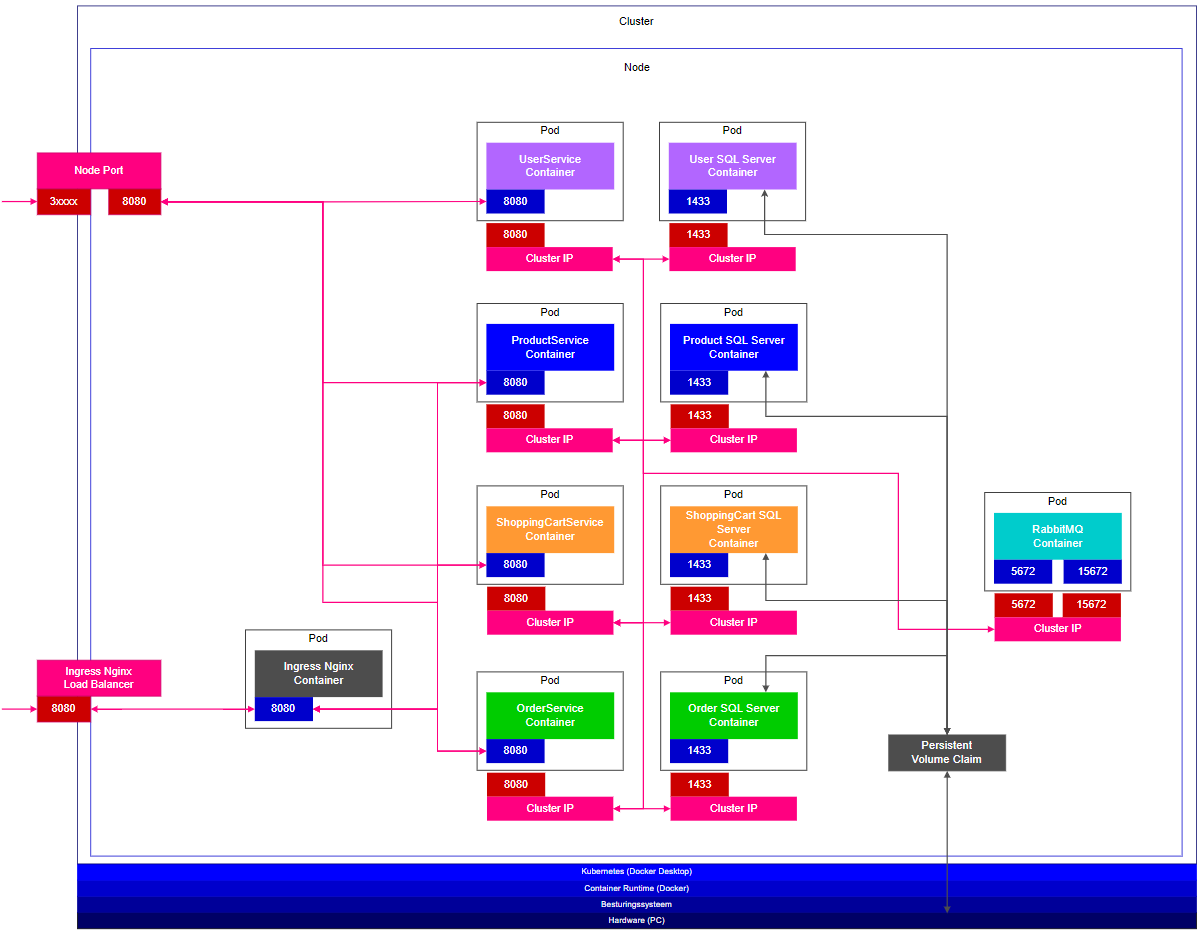
\includegraphics[width=1\textwidth]{BPMicro.png}
	\caption[Voorstelling van de microservices-architectuur voor de PoC.]{\label{fig:BPMicro}Voorstelling van de microservices-architectuur voor de PoC.\linebreak}
\end{figure}

De projectstructuur van de microservices is grotendeels gelijk aan die van de monolithische applicatie. Behalve de \texttt{UserService}, die is ontwikkeld in JavaScript en het Express framework. Deze keuze werd gemaakt om de flexibiliteit in technologiekeuze te demonstreren, zoals eerder besproken in de sectie over \hyperref[sec:flexibiliteit_technologiekeuze]{flexibiliteit in technologiekeuze}.

Daarnaast bevatten de \texttt{ShoppingCartService} en de \texttt{OrderService} een aantal extra mappen voor het afhandelen van asynchrone communicatie. Deze mappen bevatten de configuratie van RabbitMQ, event-handlers en data transfer objecten specifiek voor de asynchrone communicatie tussen beide services.

\subsection{Interservice communicatie}

In een microservices-architectuur is de communicatie tussen verschillende services een essentieel onderdeel om een goed functionerende applicatie te ontwerpen. Deze communicatie kan op twee manieren verlopen: synchroon of asynchroon. In volgend hoofdstuk worden beide vormen van communicatie getoond aan de hand van de implementatie.

\subsubsection{Synchrone communicatie}

Binnen de microservices versie van de applicatie wordt synchrone communicatie bijvoorbeeld gebruikt tussen de \texttt{ProductService} en de \texttt{ShoppingCartService}. Wanneer de \texttt{ShoppingCartService} een product wil toevoegen aan een winkelwagen, wordt eerst een HTTP-request verstuurd naar de \texttt{ProductService} om te controleren of het product bestaat. Pas nadat de \texttt{ShoppingCartService} een antwoord krijgt wordt er verder gegaan. Dit zorgt er wel voor dat de 2 services afhankelijker van elkaar worden.
\medskip

\begin{lstlisting}[style=mystyleA, caption=ShoppingCartsController.cs (fragment)(Microservice), label=lst:MicroSCCPUT]
[Route("api/[controller]")]
[ApiController]
public class ShoppingCartsController : ControllerBase
{
	private readonly IShoppingCartRepo _repository;
	private readonly IMapper _mapper;
	private readonly IProductDataClient _productClient;
	
	public ShoppingCartsController(IShoppingCartRepo repository, IMapper mapper, IProductDataClient productClient)
	{
		_repository = repository;
		_mapper = mapper;
		_productClient = productClient;
	}
	
	[HttpPut("{productId}")]
	public async Task<ActionResult> AddProductToCart(int productId)
	{
		Console.WriteLine("--> Adding a product...");
		
		var userIdHeader = Request.Headers["UserId"].FirstOrDefault();
		if (string.IsNullOrEmpty(userIdHeader))
			return BadRequest("UserId header is required");
		
		if (!int.TryParse(userIdHeader, out int userId))
			return BadRequest("UserId header must be a valid integer");
		
		var productExists = await _productClient.DoesProductExists(productId);
		if (!productExists)
			return BadRequest($"Product with id {productId} does not exist");
		
		var response = await _repository.AddProductToCart(userId, productId);
		
		if (response)
			return Ok($"Product {productId} added to cart for user {userId}");
		else
			return BadRequest($"Failed to add product {productId} to cart for user {userId}");
	}
}
\end{lstlisting}

\begin{lstlisting}[style=mystyleA, caption=ProductDataClient.cs (fragment)(Microservice), label=lst:MicroProductDataCl]
public class ProductDataClient : IProductDataClient
{
	private readonly HttpClient _httpClient;
	private readonly IConfiguration _configuration;
	
	public ProductDataClient(HttpClient httpClient, IConfiguration configuration)
	{
		_httpClient = httpClient;
		_configuration = configuration;
	}
	
	public async Task<bool> DoesProductExists(int productId)
	{
		Console.WriteLine("--> Does product exists?");
		var response = await _httpClient.GetAsync($"{_configuration["ProductService"]}/{productId}");
		if (response.IsSuccessStatusCode)
			return true;
		return false;
	}
}
\end{lstlisting}

\subsubsection{Asyncrhone communicatie}

Asynchrone communicatie is terug te vinden tussen de \texttt{OrderService} en de \texttt{ShoppingCartService}. Deze moeten namelijk niet wachten op een antwoord van de andere service om ver te kunnen met hun intern proces. Wanneer een bestelling wordt geplaatst, wordt er via RabbitMQ een bericht verstuurd dat een bestelling met betrekking tot een bepaalde winkelwagen is aangemaakt. De \texttt{ShoppingCartService} ontvangt dit bericht en verwijdert de desbetreffende winkelwagen.
\medskip

\begin{lstlisting}[style=mystyleA, caption=OrdersController.cs (fragment)(Microservice), label=lst:MicroOrdersC]
[Route("api/[controller]")]
[ApiController]
public class OrdersController : ControllerBase
{	
	[HttpPost]
	public async Task<ActionResult<OrderReadDto>> CreateOrder()
	{
		Console.WriteLine("--> Placing an order...");
		try
		{
			// Get the user ID from the logged-in user
			var userIdHeader = Request.Headers["UserId"].FirstOrDefault();
			if (string.IsNullOrEmpty(userIdHeader))
				return BadRequest("UserId header is required");
			if (!int.TryParse(userIdHeader, out int userId))
				return BadRequest("UserId header must be a valid integer");
			
			var shoppingCartDto = await _dataClient.GetShoppingCartContent(userId);
			var orderToPlace = _mapper.Map<Order>(shoppingCartDto);
			orderToPlace.Status = "Verwerking";
			orderToPlace.TotalPrice = orderToPlace.Items.Sum(i => i.Price);
			
			await _repository.PlaceOrder(orderToPlace);
			
			var orderReadDto = _mapper.Map<OrderReadDto>(orderToPlace);
			
			// Tell the ShoppingCartService about the order
			try
			{
				var orderPublishedDto = _mapper.Map<OrderPublishedDto>(orderReadDto);
				orderPublishedDto.Event = "Order_Published";
				await _messageBusClient.PublishNewOrder(orderPublishedDto);
			}
			catch (Exception ex)
			{
				Console.WriteLine($"--> Could not send asynchronously: {ex.Message}");
			}
			
			return CreatedAtRoute(nameof(GetOrderById), new { OrderId = orderReadDto.Id }, orderReadDto);
		}
		catch (Exception ex)
		{
			return BadRequest(ex.Message);
		}
	}
}
\end{lstlisting}

\begin{lstlisting}[style=mystyleA, caption=MessageBusClient.cs (Microservice), label=lst:MicroMessageBusCl]
public class MessageBusClient : IMessageBusClient
{
	private readonly IConfiguration _config;
	private readonly ConnectionFactory _factory;
	private IConnection? _connection;
	private IChannel? _channel;
	
	public MessageBusClient(IConfiguration config)
	{
		_config = config;
		_factory = new ConnectionFactory()
		{
			HostName = _config["RabbitMQHost"],
			Port = int.Parse(_config["RabbitMQPort"])
		};
	}
	
	public async Task InitializeAsync()
	{
		try
		{
			_connection = await _factory.CreateConnectionAsync();
			_channel = await _connection.CreateChannelAsync();
			
			await _channel.ExchangeDeclareAsync(exchange: "trigger", type: ExchangeType.Fanout);
			
			_connection.ConnectionShutdownAsync += RabbitMQ_ConnectionShutdown;
			
			Console.WriteLine("--> Connected to MessageBus");
		}
		catch (Exception ex)
		{
			Console.WriteLine($"--> Could not connect to message bus: {ex.Message}");
		}
	}
	
	public async Task PublishNewOrder(OrderPublishedDto orderPublishedDto)
	{
		var message = JsonSerializer.Serialize(orderPublishedDto);
		
		if (_channel == null || _connection == null)
		{
			throw new InvalidOperationException("RabbitMQ connection is not initialized");
		}
		
		if (_connection.IsOpen)
		{
			Console.WriteLine("--> RabbitMQ Connection Open, sending something...");
			// Put the OrderPublishedDto onto the MessageBus
			await SendMessage(message);
		}
		else
		{
			Console.WriteLine("--> RabbitMQ Connection is closed, not sending");
		}
	}
	
	private async Task SendMessage(string message)
	{
		var body = Encoding.UTF8.GetBytes(message);
		
		await _channel.BasicPublishAsync(
			exchange: "trigger",
			routingKey: "",
			body: body
		);
		Console.WriteLine($"--> We have sent {message}");
	}
	
	public void Dispose()
	{
		System.Console.WriteLine("--> MessageBus Disposed");
		if (_channel.IsOpen)
		{
			_channel.CloseAsync();
			_connection.CloseAsync();
		}
	}
	
	private async Task RabbitMQ_ConnectionShutdown(object sender, ShutdownEventArgs e)
	{
		Console.WriteLine("--> RabbitMQ Connection Shutdown");
		await Task.CompletedTask;
	}
}
\end{lstlisting}

\begin{lstlisting}[style=mystyleA, caption=MessageBusSub.cs (Microservice), label=lst:MicroMessageBusSb]
public class MessageBusSub
{
	private readonly IConfiguration _config;
	private readonly IEventProcessor _eventProcessor;
	private readonly ConnectionFactory _factory;
	private IConnection _connection;
	private IChannel _channel;
	private QueueDeclareOk _queue;
	private string _queueName;
	
	public MessageBusSub(IConfiguration config, IEventProcessor eventProcessor)
	{
		_config = config;
		_eventProcessor = eventProcessor;
		_factory = new ConnectionFactory
		{
			HostName = _config["RabbitMQHost"],
			Port = int.Parse(_config["RabbitMQPort"])
		};
	}
	
	public async Task InitializeRabbitMQAsync()
	{
		try
		{
			_connection = await _factory.CreateConnectionAsync();
			_channel = await _connection.CreateChannelAsync();
			
			await _channel.ExchangeDeclareAsync(exchange: "trigger", type: ExchangeType.Fanout);
			
			_queue = await _channel.QueueDeclareAsync();
			_queueName = _queue.QueueName;
			await _channel.QueueBindAsync(queue: _queueName, exchange: "trigger", routingKey: "");
			
			Console.WriteLine("--> Listening to the Message Bus...");
		}
		catch (Exception ex)
		{
			Console.WriteLine($"--> Could not connect to message bus: {ex.Message}");
		}
		
		WaitForEvents();
	}
	
	private async void WaitForEvents()
	{
		var consumer = new AsyncEventingBasicConsumer(_channel);
		
		consumer.ReceivedAsync += (model, ea) =>
		{
			Console.WriteLine("--> Event Received!");
			byte[] body = ea.Body.ToArray();
			var message = Encoding.UTF8.GetString(body);
			_eventProcessor.ProcessEvent(message);
			return Task.CompletedTask;
		};
		
		await _channel.BasicConsumeAsync(queue: _queueName, autoAck: true, consumer: consumer);
	}
}
\end{lstlisting}

\begin{lstlisting}[style=mystyleA, caption=EventProcessor.cs (Microservice), label=lst:MicroEventPrc]
public class EventProcessor : IEventProcessor
{
	private readonly IServiceScopeFactory _scopeFactory;
	private readonly IMapper _mapper;
	
	public EventProcessor(IServiceScopeFactory scopeFactory, IMapper mapper)
	{
		_scopeFactory = scopeFactory;
		_mapper = mapper;
	}
	
	public async Task ProcessEvent(string message)
	{
		var eventType = DetermineEvent(message);
		
		switch (eventType)
		{
			case EventType.OrderPublished:
				await RemoveShoppingCart(message);
				break;
			default:
				break;
		}
	}
	
	private EventType DetermineEvent(string notificationMessage)
	{
		Console.WriteLine("--> Determining Event");
		
		var eventType = JsonSerializer.Deserialize<GenericEventDto>(notificationMessage);
		
		switch (eventType.Event)
		{
			case "Order_Published":
				Console.WriteLine("--> Order Published Event Detected");
				return EventType.OrderPublished;
			default:
				Console.WriteLine("--> Could not determine the event type");
				return EventType.Undetermined;
		}
	}
	
	private async Task RemoveShoppingCart(string orderPublishedMessage)
	{
		using var scope = _scopeFactory.CreateScope();
		var repo = scope.ServiceProvider.GetRequiredService<IShoppingCartRepo>();
		
		var orderPublishedDto = JsonSerializer.Deserialize<OrderPublishedDto>(orderPublishedMessage);
		var shoppingCartId = orderPublishedDto.ShoppingCartId;
		var userId = orderPublishedDto.UserId;
		
		try
		{
			if (repo.ShoppingCartExists(shoppingCartId, userId))
			{
				var cart = await repo.GetCart(userId);
				repo.DeleteCart(cart);
				Console.WriteLine("--> ShoppingCart removed");
			}
			else
			{
				Console.WriteLine("--> ShoppingCart does not exists...");
			}
		}
		catch (Exception ex)
		{
			Console.WriteLine($"--> Could not remove ShoppingCart: {ex.Message}");
		}
	}
}
\end{lstlisting}

%% TODO: In dit hoofstuk geef je een korte toelichting over hoe je te werk bent
%% gegaan. Verdeel je onderzoek in grote fasen, en licht in elke fase toe wat
%% de doelstelling was, welke deliverables daar uit gekomen zijn, en welke
%% onderzoeksmethoden je daarbij toegepast hebt. Verantwoord waarom je
%% op deze manier te werk gegaan bent.
%% 
%% Voorbeelden van zulke fasen zijn: literatuurstudie, opstellen van een
%% requirements-analyse, opstellen long-list (bij vergelijkende studie),
%% selectie van geschikte tools (bij vergelijkende studie, "short-list"),
%% opzetten testopstelling/PoC, uitvoeren testen en verzamelen
%% van resultaten, analyse van resultaten, ...
%%
%% !!!!! LET OP !!!!!
%%
%% Het is uitdrukkelijk NIET de bedoeling dat je het grootste deel van de corpus
%% van je bachelorproef in dit hoofstuk verwerkt! Dit hoofdstuk is eerder een
%% kort overzicht van je plan van aanpak.
%%
%% Maak voor elke fase (behalve het literatuuronderzoek) een NIEUW HOOFDSTUK aan
%% en geef het een gepaste titel.

